\chapter{Introduction}
\graphicspath{ {chapters/Introduction/} }

Nowadays in the manufacturing industry most of the production is automated. This is being referred to as the Industry 3.0 or the third industrial revolution. \\ 

\begin{figure}
	\caption{Industry 4.0 \cite{pictIndustry40}}
	\centering
	  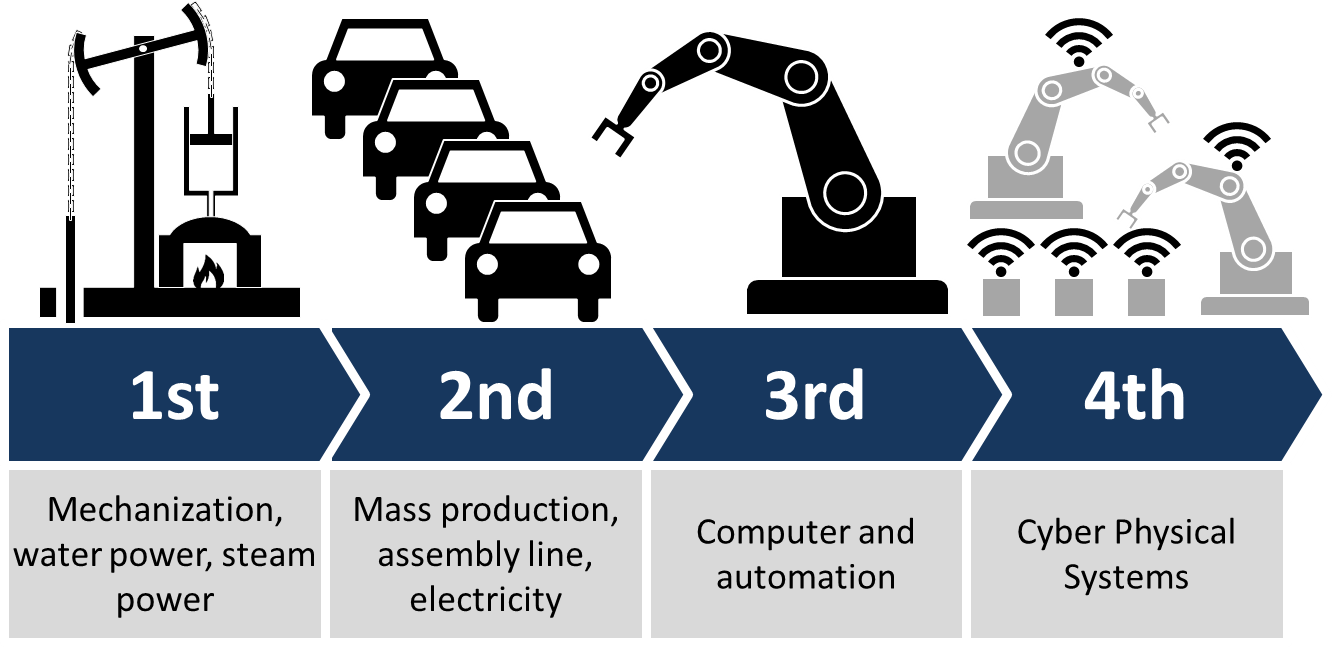
\includegraphics[width=0.5\textwidth]{industry-40.png}
\end{figure}

	
 Parts of the product are created and assembled in robotic cells or robotic assembly lines. When developing a new product the engineers usually create a CAD model of the product and based on that build prototypes. When refined a different engineering team is tasked with designing an assembly line that could mass produce the parts and assemble them together. \\
 
It widely is believed that the future (Industry 4.0) will revolve around automation and data exchange. These so called \"smart factories\" should be able to manufacture goods with unprecedented effectivity and ease. Beyond Industry 4.0, smart factories will only reach their potential when we'll be able to design a product and then just let a factory manufacture it for us without human intervention.   

Currently, assembly lines are designed in a specific type of CAD software, which allows the simulation of the full assembly sequence. This way the engineers can validate the reachability and collision clearance of the prepared line, including human factors. One example of such software is the Tecnomatix suite by SIEMENS. Tecnomatix Process Simulate is an industry leading software for digital manufacturing, used by the likes of Blumenbecker or Skoda \ref{source of this information}. \\ 

When designing an assembly line for a product the focus is on the successful creation of the product, which in itself is a no mean feat. Then searching for the optimal layout of the robots and schedule of the tasks that need to be executed for the desired result is an inhuman task. 

\section{Motivation}

Rather than focusing the question of the layout of the robots which would require knowing the available space, layout of the factory, location of the power outlets and so on. Since this problem would be bigger than one lifetime of work, we need to apply the divide and conquer principle. Rather than looking at the whole problem this thesis tries to tackle a smaller part, hoping that other research could build on it. The goal is to take the human design of the assembly line and apply a mathematical model to find the optimal schedule which could be used to marginally improve the effectivity of the line. \\

The schedule could be optimized with different goals in mind, for example: cycle time or energy consumption (leveraging the robots sleep modes). This work focuses on building the bridge between the design tool and a MILP model which can be swapped out. 

Based on the energy usage of manufacturing companies \ref{source and some numbers} the savings could range in millions of dollars per year.

\section{Related Work}

tutorial pro process simulate + ref + popis

energy simulation clanek kluku + ref + popis

 

There are multiple articles regarding the optimization algorithms used. For this reason I chose to make this work focus on the practical part of connecting the optimization algorithm and the tool itself.


strukturovane co se tyce algoritmu, toolu, atd\ldots vypichnuti thedulezitych veci co vyuzije sekce Contribution)

\section{Contribution and Outline}

vzhledem k existujicim pracem neexistuje takova a takova prace + popis inovaci, a v pristi sekci bude ... a pak ... atd ...

This work could bridge the world of theoretical improvements and algorithms with the practical world.; 

\section{Problem Statement}

In the assembly line we consider robots as the main actor. Humans can be also counted as a robot for the optimization purposes. Every robot as a set of actions that he needs to perform, and the action can also depend on other action. 
- Mejme n robotu a mejme graf co popisuje operace\ldots 
